\chapter{Presentation of the Tasks Performed}
\label{ch:tasks}

This chapter details the technical work carried out during the
internship: the architecture of the research pipeline, the construction
of each of its modules, and --- occupying the larger part of the
internship --- the successive redesign cycles that experimental evidence
forced upon it.

\section{Global Pipeline Architecture}

\subsection{Delivered Functional Flow}

The system is organised as a single linear data flow, split across two
independent executable entry points that share a common construction
layer:

\begin{enumerate}[leftmargin=*]
  \item \file{ingestion.py} downloads the RSNA dataset and exposes it as
        an \texttt{RSNACXRDataset}.
  \item \file{pipeline.py}'s \texttt{build\_common()} constructs the
        dataset, the frozen models and the generator. Both entry points
        call it, which guarantees that training and evaluation operate on
        \emph{identical} objects.
  \item \file{src/models.py} loads and freezes the classifier, the
        PSPNet segmenter and the YOLOv8 feature extractor.
  \item \file{src/generator.py} and \file{factory/finetuning.py}
        adapt the Stable Diffusion UNet to the radiograph domain via
        LoRA.
  \item \file{factory/environment.py} and \file{factory/ppo.py} train
        two directional PPO policies.
  \item \file{eval_main.py} reloads the checkpoints and runs
        \file{src/metrics.py} and \file{src/diff_viz.py}.
\end{enumerate}

Alongside this main path sit two diagnostic tools that never participate
in training: \file{heldout_validation.py} and
\file{check_classifier_localization.py}.

\subsection{Splitting Training from Evaluation}
\label{sec:walltime}

The pipeline was originally a single process, \file{main.py}, that
trained both policies and then evaluated them. This design failed
concretely. Job \textbf{17644171} completed PPO training, wrote both
policies to disk, and was then killed at the 24-hour walltime boundary
partway through evaluation. No metrics were produced, and --- critically
--- no entry point existed that could reload the surviving policies. A
full training run had to be repeated to recover a number that the
finished policies could already have produced.

The pipeline was restructured in response. \file{main.py} now performs
Steps~1--5 (training) and terminates after writing checkpoints;
\file{eval_main.py} performs Steps~6--6B (evaluation) as a separate
process, failing fast with an explicit message if the expected policy
checkpoints are absent. Beyond removing the walltime hazard, this gives
evaluation the property of being freely repeatable: metric fixes,
different sample sizes and regenerated plots no longer cost a training
run.

This split also created a subtler risk, addressed by
\file{smoke_test_eval.py}: with training and evaluation in one process,
a checkpoint that fails to reload correctly in a \emph{cold} process is
invisible, because the objects are already in memory. The evaluation
smoke test exercises precisely that cold-reload path.

\section{Data and Generator Work}

\subsection{Dataset Preparation}

\file{ingestion.py} retrieves the RSNA Pneumonia Detection Challenge
corpus and derives a binary label from the challenge's bounding-box
annotations: a study is positive if any box marks lung opacity, negative
otherwise. DICOM files are decoded, min--max normalised to $[0,1]$ and
resized to $256\times256$. The loaded corpus comprises \textbf{26{,}684
studies}: 6{,}012 positive and 20{,}672 negative.

\subsection{Class Imbalance and Balanced Sampling}

The $22.5\%$ positive rate is a problem for denoising fine-tuning, which
is class-conditional: trained on the natural distribution, the generator
sees pneumonia-positive radiographs less than a quarter of the time and
learns a correspondingly weaker conditional model for exactly the class
the harder edit direction must synthesise.

\file{factory/finetuning.py} addresses this with a
\file{WeightedRandomSampler} (\file{_build_balanced_sampler}),
weighting each sample by the inverse frequency of its class so that each
epoch presents roughly balanced classes. The function fails loudly rather
than silently degrading if a class is absent from the dataset.

\subsection{LoRA Fine-Tuning}

The SD1.5 UNet is adapted with rank-16 LoRA adapters
($\alpha = 16$, dropout $0.05$) inserted into the attention projections
\texttt{to\_q}, \texttt{to\_k}, \texttt{to\_v} and \texttt{to\_out.0},
trained on the standard $\epsilon$-prediction denoising objective for 30
epochs at learning rate $10^{-4}$. Class conditioning replaces SD1.5's
text encoder entirely: a small \texttt{cond\_proj} MLP maps the target
class and a pooled latent summary to a single cross-attention
conditioning token.

The training loop checkpoints every epoch and resumes from
\file{checkpoints/finetuning_latest.pt}, a necessity in a walltime-bounded
batch environment --- the log of the most recent run shows it correctly
detecting a completed 30-epoch fine-tune and skipping straight past
Step~4.

An earlier iteration used rank~8; its checkpoints are preserved under
\file{checkpoints/archive_v1_rank8/} for comparison.

\subsection{Gradient-Guided DDIM Sampling}

Counterfactual generation (\file{src/generator.py}) performs a partial
forward-then-reverse DDIM trajectory, whose length is set by a
\texttt{strength} fraction of the $T_{\text{diff}}=50$ step schedule. At
each reverse step, two gradient terms are injected into the predicted
clean latent $\hat z_0$:

\[
  \Delta z_0 = -\,w(i)\,\alpha_{\text{cls}}\,
  \nabla_{\hat z_0}\mathcal{L}_{\text{cls}}
  \;-\; w(i)\,\alpha_{\text{pres}}\,\nabla_{\hat z_0}
  \big(\text{seg-weighted L1} + \eta\,\text{obj-det MSE}\big)
\]

The first term drives the classifier toward the target class; the second
penalises departure from the original image, both in anatomy
(segmentation-weighted L1) and in object-detector feature space. The
factor $w(i)$ is a linear ramp that rises from 0 to 1 starting at a
policy-chosen fraction of the trajectory, replacing an earlier hard
on/off guidance switch whose discontinuity destabilised sampling.

\subsection{The Background Lock}

Gradient guidance alone provides no guarantee about \emph{where} an edit
lands. The generator therefore applies a hard spatial constraint adapted
from RePaint~\cite{lugmayr2022repaint} and Blended Latent
Diffusion~\cite{avrahami2022blended}: at every denoising step, the latent
\emph{outside} a dilated, Gaussian-feathered lung-segmentation mask is
overwritten with the original image's latent, forward-noised to the
current timestep (and clean at the final step).

This is a structural guarantee rather than a soft penalty. Content
outside the lung field cannot be repainted by the sampler regardless of
how the guidance gradient behaves; it can only collapse to the VAE's
reconstruction floor. Without it, an aggressive \texttt{strength}
schedule repaints the entire thorax.

\section{Reinforcement-Learning Control}

\subsection{Environment Design}

\texttt{MedicalCounterfactualEnv} (\file{factory/environment.py}) exposes
the sampling procedure as a Gym-style MDP. An episode begins by sampling
a ``far'' image --- one the classifier scores more than
\texttt{FAR\_THRESHOLD}$=0.5$ away from the target class. The most recent
run logs the resulting pool: \textbf{15{,}267 of 26{,}684 images} qualify
for the \ntop{} direction, split into 15{,}243 for rollouts and 24
withheld for a validity probe.

The observation concatenates the flattened original and current latents,
a normalised step index, the current $|f(x_t) - c|$, the target class,
and the flattened lung mask --- $73{,}731$ dimensions in total, as logged
at policy construction. Episodes terminate when
$|f(x_t) - c| < \varepsilon_{\text{stop}} = 0.08$ or the step budget
$T = 8$ is exhausted.

\subsection{Action Space}

The policy emits a 9-dimensional continuous action at each step, mapped
through sigmoid transforms onto bounded control ranges:

\begin{table}[h]
\centering
\caption[PPO action space]{PPO action space (\file{factory/environment.py},
\texttt{MedicalCounterfactualEnv.step}).}
\label{tab:actions}
\begin{tabular}{@{}clc@{}}
\toprule
\textbf{Dim} & \textbf{Controls} & \textbf{Range} \\
\midrule
$a_0$ & DDIM strength                                  & $[0.20,\,0.70]$ \\
$a_1$ & classifier-guidance scale                      & $[0.30,\,1.20]$ \\
$a_2$ & preservation-guidance scale                    & $[0.30,\,1.50]$ \\
$a_3$ & stop signal $\tau_t$                           & $[0,\,1]$ \\
$a_4, a_5$ & one extra refinement pass each (Bernoulli gates) & $\{0,1\}$ \\
$a_6$ & per-pass strength boost                        & $[0.85,\,1.15]$ \\
$a_7$ & guidance bias (classifier vs.\ preservation)   & $[0.70,\,1.30]$ \\
$a_8$ & guidance ramp-up start fraction                & $[0.10,\,0.50]$ \\
\bottomrule
\end{tabular}
\end{table}

The classifier-guidance ceiling in $a_1$ was deliberately narrowed during
development, from a maximum of $3.0$ down to $1.2$. At the original
ceiling a single step could brute-force the classifier flip, and episodes
collapsed to an average length of exactly $1.00$ --- leaving PPO with no
temporal structure from which to learn credit assignment. Capping the
per-step push forces the flip to be reached over several steps, which is
what makes the problem a sequential decision problem at all.

\subsection{Actor-Critic Architecture}

\texttt{PPOActorCritic} (\file{factory/ppo.py}) uses a convolutional
trunk over the latent-shaped portion of the observation (three
\texttt{Conv2d} layers, $32\to64\to128$ channels, followed by a
256-unit MLP head that also consumes the scalar observation components).
This trunk feeds four heads: a Gaussian policy head with a
\textbf{learnable per-dimension \texttt{log\_std}} parameter, a value
head, and three auxiliary heads predicting feasibility, progress and the
stop decision, each trained with its own auxiliary loss.

Making \texttt{log\_std} a learned parameter rather than a fixed
schedule lets the agent modulate its own exploration per action
dimension. The resulting policy is compact: \textbf{197{,}910
parameters}, against an observation of $73{,}731$ dimensions.

Advantages are computed with GAE~\cite{schulman2016gae}
($\gamma = 0.99$, $\lambda = 0.95$) and the policy updated with the
clipped PPO objective~\cite{schulman2017ppo} (clip $0.2$, value
coefficient $0.5$, entropy coefficient $0.01$).

\subsection{Two Directional Policies}

The environment is constructed around a single fixed target class, so two
policies are trained independently: one for normal$\rightarrow$pneumonia
($c=1$) and one for pneumonia$\rightarrow$normal ($c=0$). They share the
same fine-tuned generator but specialise their sampling schedules. A
single target-conditioned policy would be architecturally cleaner, and is
identified in Section~\ref{sec:future} as future work.

\section{Iterative Debugging and Redesign}

The chronology below is reconstructed from the repository's commit
history and from the design rationale recorded in \file{config.py}, which
was maintained as a running experimental log throughout the internship.

\subsection{Diagnosis: the Reward Was Almost Entirely a Flip Bonus}

Early counterfactuals changed between 66\% and 75\% of all pixels ---
diffuse, whole-image edits rather than localised lesions. Decomposing the
reward actually obtained by the v1 policy (reconstructed from job
\textbf{17648782}, which logged \texttt{avg\_return}$=33.931$ at
\texttt{avg\_ep\_len}$=1.00$) explained why:

\begin{table}[h]
\centering
\caption[v1 reward decomposition]{Reward decomposition of the v1 policy, reconstructed from job 17648782.
The terminal flip bonuses accounted for 93\% of the return; preservation was
numerically negligible.}
\label{tab:v1reward}
\begin{tabular}{@{}lrr@{}}
\toprule
\textbf{Reward term} & \textbf{Contribution} & \textbf{Share} \\
\midrule
\Rterm{hit} $\times 6$ and \Rterm{stop} $\times 8$ & $+14.00$ & 93\% \\
\Rterm{prog} $\times 1.5$                          & $+1.40$  & 9\% \\
\Rterm{pres} $\times 0.5$                          & $-0.21$  & $-1.4$\% \\
\Rterm{fid} $\times 0.5$ (on MSE $0.0033$)         & $-0.0016$& $-0.01$\% \\
\bottomrule
\end{tabular}
\end{table}

The flip bonus \emph{was} the reward. Preservation contributed roughly
one part in a hundred and image fidelity one part in ten thousand, so the
optimal policy was to flip the classifier by any means available and stop
immediately. Three changes followed:

\begin{itemize}[leftmargin=*]
  \item \textbf{Rebalancing.} The terminal bonuses were cut
        ($\lambda_{\text{hit}}$ and $\lambda_{\text{stop}}$ from 6 and 8
        down to 2 each) and the preservation weight raised
        ($\lambda_{\text{pres}}$ from 0.5 to 3.0), targeting a roughly
        40/40/20 split between flip, preservation and progress.
  \item \textbf{L2 $\rightarrow$ L1 fidelity penalty.} \Rterm{fid} was
        computed as a mean squared error. L2 prefers many small changes
        over few large ones --- it was \emph{actively rewarding} the
        diffuse failure mode being diagnosed. Switching to L1, which is
        sparsity-inducing, required rescaling $\lambda_{\text{fid}}$ from
        0.5 to 2.0, since L1 is roughly $25\times$ larger numerically at
        these magnitudes.
  \item \textbf{Episode-origin anchoring.} With
        \texttt{ANCHOR\_TO\_EPISODE\_ORIGIN}, the background lock and the
        preservation targets are anchored to the episode's \emph{original}
        image rather than to the previous refinement pass's output.
        Anchoring to the previous pass allows unbounded drift over an
        episode; anchoring to the origin restores the Markov property and
        forces the policy to refine rather than to blast.
\end{itemize}

\subsection{A Reward-Scaling Bug in the Asymmetry Correction}

The \ntop{} direction is empirically harder than \pton{}, and was
originally compensated with a $2.25\times$ \texttt{direction\_scale}
boost on its reward. The scale was found to be applied only to the
progress terms and not to \Rterm{fid} or \Rterm{pres} --- meaning
preservation was effectively $2.25\times$ \emph{less} important on
precisely the direction that was already producing the most diffuse
edits.

Applying the scale uniformly across all reward terms corrected the
relative weighting. It is worth stating explicitly, as the code's own
change log does, that under PPO's per-update advantage normalisation a
uniform scalar multiplying the entire reward is close to a no-op for the
policy gradient. The fix removed a harmful \emph{relative} re-weighting;
it did not inject additional learning signal into the harder direction,
and the residual asymmetry in Chapter~\ref{ch:results} is consistent with
that.

\subsection{Grad-CAM Localisation Check}
\label{sec:gradcam_mask}

Before trusting a classifier to supply a guidance gradient, it is
necessary to establish that it responds to pathology rather than to a
global brightness or contrast shortcut --- a well-documented failure mode
of CXR classifiers, and one that would make every generated
counterfactual a mere exposure adjustment.

\file{check_classifier_localization.py} renders Grad-CAM overlays for
this purpose. The comparison between the original classifier and the
TorchXRayVision DenseNet-121 is shown in Figure~\ref{fig:gradcam}.

\begin{figure}[h]
  \centering
  \begin{subfigure}[b]{0.48\textwidth}
    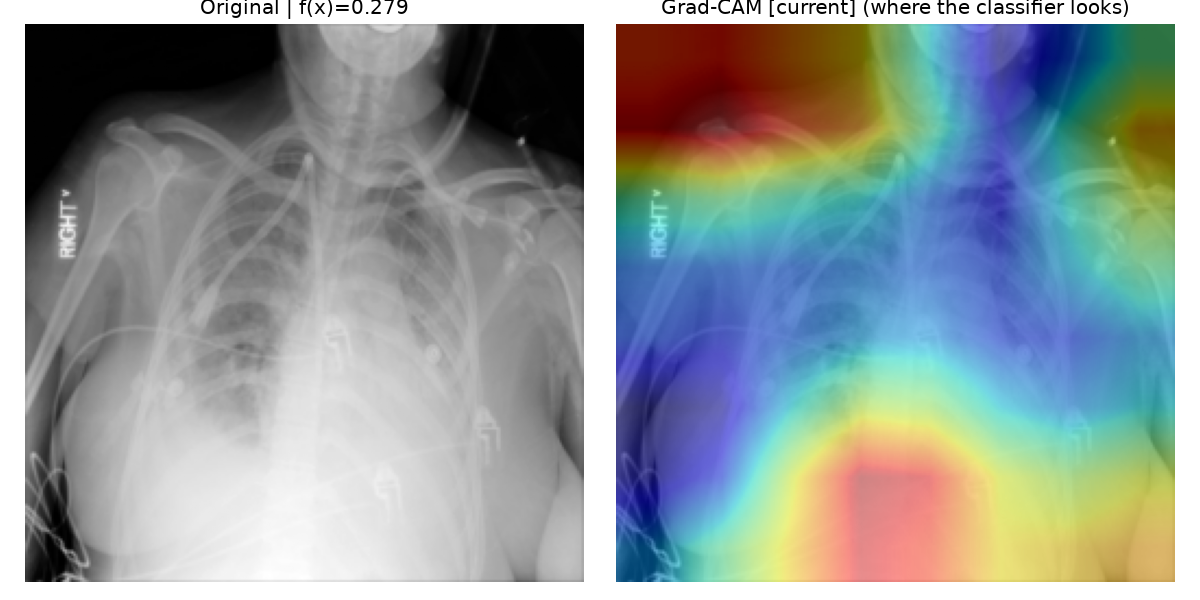
\includegraphics[width=\textwidth]{gradcam_current_0.png}
    \caption{Original classifier.}
  \end{subfigure}\hfill
  \begin{subfigure}[b]{0.48\textwidth}
    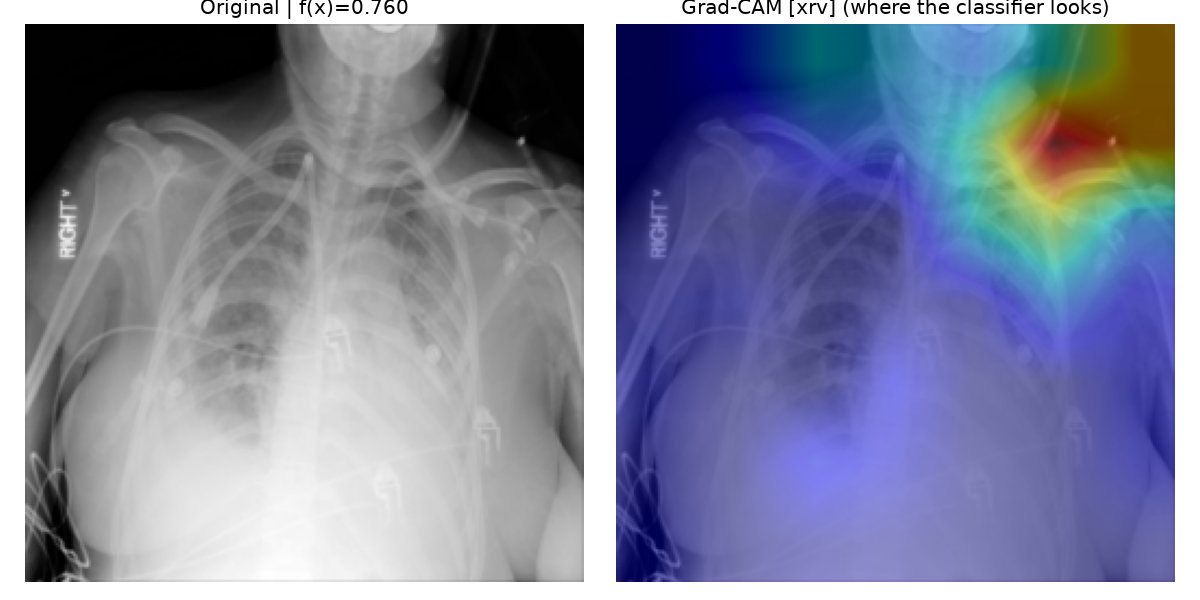
\includegraphics[width=\textwidth]{gradcam_xrv_0.png}
    \caption{TorchXRayVision DenseNet-121.}
  \end{subfigure}
  \caption[Grad-CAM localisation diagnostic]{Grad-CAM localisation diagnostic, one representative case from
  the six pairs written to \file{outputs/gradcam_check/}. This diagnostic
  motivated the replacement of the project's own ResNet-18 classifier
  (\file{checkpoint/classifier.pt}) with the pretrained TorchXRayVision
  DenseNet-121 as the guidance model.}
  \label{fig:gradcam}
\end{figure}

The same Grad-CAM implementation was subsequently promoted from a
diagnostic to a \emph{constraint}. With \texttt{USE\_GRADCAM\_MASK}, the
map is normalised at its 99th percentile, raised to a power
$\gamma = 0.75$, floored at $0.15$ and Gaussian-blurred, then used to
modulate the edit budget spatially --- so the agent may edit freely where
the classifier attends and only marginally elsewhere.

Enabling this required an ensemble-aware Grad-CAM path
(\texttt{gradcam.ensemble\_grad\_cam}). Without it, resolving the target
layer on an ensemble walks \texttt{named\_modules()} and silently returns
the \emph{first member's} feature block, producing a single-model CAM
mislabelled as the ensemble's. This is recorded in \file{config.py} as
verified behaviour rather than a suspicion.

\subsection{Sparsity Reward with Annealed Ramp}

Even after the reward rebalance, measured edit concentration --- the
share of total $|\Delta|$ carried by the top 5\% of pixels --- stood at
$0.282$ (\ntop{}) and $0.297$ (\pton{}) against a uniform baseline of
$0.05$. A concentrated core existed, but most of the edit mass sat in a
diffuse tail.

An explicit L1 sparsity reward term was added to target that tail, with
two refinements. First, it is \emph{annealed}: the weight is zero for the
first 20\% of updates, ramps linearly to its target of $2.0$ between 20\%
and 60\%, and is constant thereafter, so the policy first learns a
reliable flip and only then is pressured toward minimal edits.
Second, with \texttt{SPARSITY\_OUTSIDE\_CAM\_ONLY} the penalty is
weighted by $(1-\text{CAM})$, penalising only edit mass \emph{outside}
the attended region --- a plain L1 would also penalise the concentrated
core that the method is trying to keep.

A safeguard accompanies the ramp: validity is probed on a held-out set
every 10 updates, and the ramp freezes if it drops more than 8 points
below its pre-ramp baseline. The size of that held-out set was chosen
rather than guessed. Validity is a fraction over $N$ images, so its
resolution is $1/N$; at $N=8$ a single image moves it by 12.5 points and
the freeze would latch on noise in essentially every run. $N=24$ gives
4.2 points per image, placing the 8-point tolerance safely above the
noise floor.

\subsection{Held-Out Validation and the Move to an Ensemble}
\label{sec:heldout_method}

The most consequential finding of the internship came from questioning
the primary metric. Counterfactual Validity was being computed with the
\emph{same} classifier that produced the guidance gradient. That number is
circular: it measures how well an optimiser optimised its own objective,
not whether the resulting image depicts disease.

\file{heldout_validation.py} was written as the independent check. It
re-scores the generated counterfactuals with TorchXRayVision classifiers
that never participated in the guidance loop, and includes an agreement
control on the \emph{original} images --- so that poor transfer cannot be
dismissed as the validators simply disagreeing about the task. It is
deliberately a separate SLURM job rather than part of
\file{eval_main.py}, and caches its generated counterfactuals so that
adding a validator costs minutes rather than hours.

The results (Chapter~\ref{ch:results}, Section~\ref{sec:heldout}) were
negative, and led directly to a redesign: the guidance signal was changed
from the single RSNA model to an \textbf{ensemble} of
\texttt{densenet121-res224-rsna} and \texttt{densenet121-res224-chex}.
The reasoning is that an adversarial direction found against one model
rarely survives against an independently trained one, so requiring
consensus makes the adversarial shortcut a substantially narrower target.
The \texttt{-chex} model was chosen specifically because its 11-head
multi-task training resists the global-brightness shortcut.

This change carries a bookkeeping obligation recorded in the
configuration: any classifier in the guidance ensemble ceases to be a
valid held-out validator. The validator set was accordingly reduced to
\texttt{nih}, \texttt{mimic\_ch} and \texttt{pc}.

\section{Experimental Infrastructure}

\subsection{Smoke Tests}

\file{smoke_test.py} and \file{smoke_test_eval.py} run the training and
evaluation paths end-to-end with deliberately tiny budgets, to surface
crashes and tensor-shape errors before a 20-hour job is queued. The
training smoke test is parameterised by an \texttt{SMOKE\_ARM}
environment variable selecting \texttt{baseline} (all new flags off,
reproducing the pre-change pipeline), \texttt{mask} (Grad-CAM constraint
only) or \texttt{all} --- the same ablation arms used to attribute
behaviour changes to individual mechanisms.

\subsection{Job Monitoring}

All batch scripts declare \texttt{--mail-type=END,FAIL} with a
notification address, so job completion and failure are reported without
polling. Each script also runs \texttt{set -euo pipefail} and performs
explicit precondition checks before loading any model weights --- the
evaluation and held-out scripts verify that the expected policy
checkpoints exist, and the held-out script additionally verifies that
each validator's weights are present in the local TorchXRayVision cache,
failing in seconds rather than after three hours of generation.

One such check encodes a non-obvious detail worth recording: the
TorchXRayVision cache filename does not always match the weight
identifier. \texttt{densenet121-res224-rsna} is cached as
\texttt{kaggle-densenet121-*.pt}, because RSNA was a Kaggle competition,
so a naive existence check for \texttt{rsna-densenet121-*} fails even on
a correctly provisioned machine.

Python is invoked unbuffered (\texttt{python -u}) throughout, so that a
job's log is readable while it is still running. In a non-interactive
environment where a stalled job cannot be inspected directly, the log is
the only diagnostic channel available.

\section{Conclusion}

This chapter has described the construction of the research pipeline and
the sequence of redesigns that experimental evidence forced: a reward
function found to be 93\% flip bonus, a fidelity penalty that rewarded
the failure mode it was meant to suppress, a direction-scaling bug that
penalised preservation on the harder direction, and --- most importantly
--- a primary metric found to be circular. The next chapter reports what
the resulting system measures, and what those measurements do and do not
establish.
